\documentclass{scrreprt}
\usepackage[bookmarks=true]{hyperref}
\usepackage{tabto}
\usepackage{epsfig}
\usepackage{epstopdf}
\hypersetup{
    pdftitle={Functional Requirement Specification},    % title
    colorlinks=true,       % false: boxed links; true: colored links
    linkcolor=blue,       % color of internal links
    citecolor=black,       % color of links to bibliography
    filecolor=black,        % color of file links
    urlcolor=purple,        % color of external links
    linktoc=page            % only page is linked
}%
\title{%
\author{
Khathutshelo Matidza 11072157\\
\and
Renaldo van Dyk 12204359\\
\and
Andreas du Preez 12207871\\
\and
Sean Hill 12221458\\
\and
Kgomotso Sito 12243273\\
\and
Hlavutelo Maluleke 12318109\\
\and
Sboniso Masilela 10416260\\
\and
Semaka Malapane 13081129\\
}
\centering
\Huge{FUNCTIONAL REQUIREMENTS\\ SPECIFICATION}\\
\vspace{2cm}
FOR\\
\vspace{2cm}
Buzz System\\
\vspace{2cm}
Mini Project Phase 1\\
GitHub\\
\LARGE\texttt{https://github.com/RenaldoV/COS301\_Group5\_a}
\vfill
\vspace{1cm}
\rule{15cm}{3pt}
}
\date{}
\usepackage{hyperref}
\begin{document}
\maketitle
\tableofcontents
\chapter{ Introduction}
This document discusses the application functionality required by users (and other stakehodlers).\\
\chapter{ Use case prioritization}
\section{Critical}
1.1 Delete\\
1.2 Read\\
1.3 Create\\
1.4 Update\\
1.5 Comment\\
\section{Important}
1.1.1 Archive post\\
2.1 Direct messages\\
3.1 The system to have a structure of some sort\\
\section{Nice-To-Have}
3.1 View visualized statistical information\\
2.1{a} The user to choose their own structure\\
2.1{b} Making use of tags\\
\chapter{Use case/Services contracts}
\NumTabs{18}
\section{Pre-Conditions}								%PRE CONDITIONS
1.1\tab{a) Post must be in database}\\
1.1\tab{b) Post must be read from database before it can be deleted}\\
1.1\tab{c) User must be logged in to the system to delete a post}\\
1.1.1\tab{a) Post must be deleted before it can be archived}\\
1.2\tab{a) Post must exist in database}\\
1.2\tab{b) User must be logged into the system to read values from database}\\
1.3\tab{a) User must be logged into the system to create posts to in database}\\
1.4\tab{a) User must be logged into the system to update the database}\\
1.4\tab{b) Before the database can be updated values must be changed}\\
2.1\tab{a} User must have registered account\\
2.1\tab{b} User must have message\\
2.1\tab{c} Message must have (a) recipient(s)\\
3.1\tab{a} User must have registered account\\
3.1\tab{b} User must have been graded\\
4.1\tab{a}) Check user status level before posting\\
4.1\tab{b}) Check word count of post before posting\\
5.1\tab{a}) Check user status level before commenting\\
5.1\tab{b}) Check word count of post before commenting\\
6.1\tab{a}) Users must be registered to be able to view content/posts according to their own structure\\
\section{Post-Conditions}								%POST CONDITIONS	
1.1\tab{a) Post will not exist in database}\\
1.1\tab{b)Post will not be visible to users}\\
1.1.1\tab{a)Post and log data will reside in an archive}\\
1.3\tab{a) Update request will be called on the new data}\\
1.3\tab{b)Post will be visible to users who are logged into the system}\\
1.4\tab{a) Post data will be inserted into database}\\
1.4\tab{b)Post will exist in database}\\
2.1\tab{a} A direct message is sent by user and recieved by recipients\\
3.1\tab{a} User views visualized statistical information\\
4.1\tab{a}) Comment should be visible to all users of that level\\
5.1\tab{a}) Posts should be organised according to tags\\
5.1\tab{b}) Registered users should be able to choose the structure in which to view tags\\
\section{Request and Results Data Structures} 
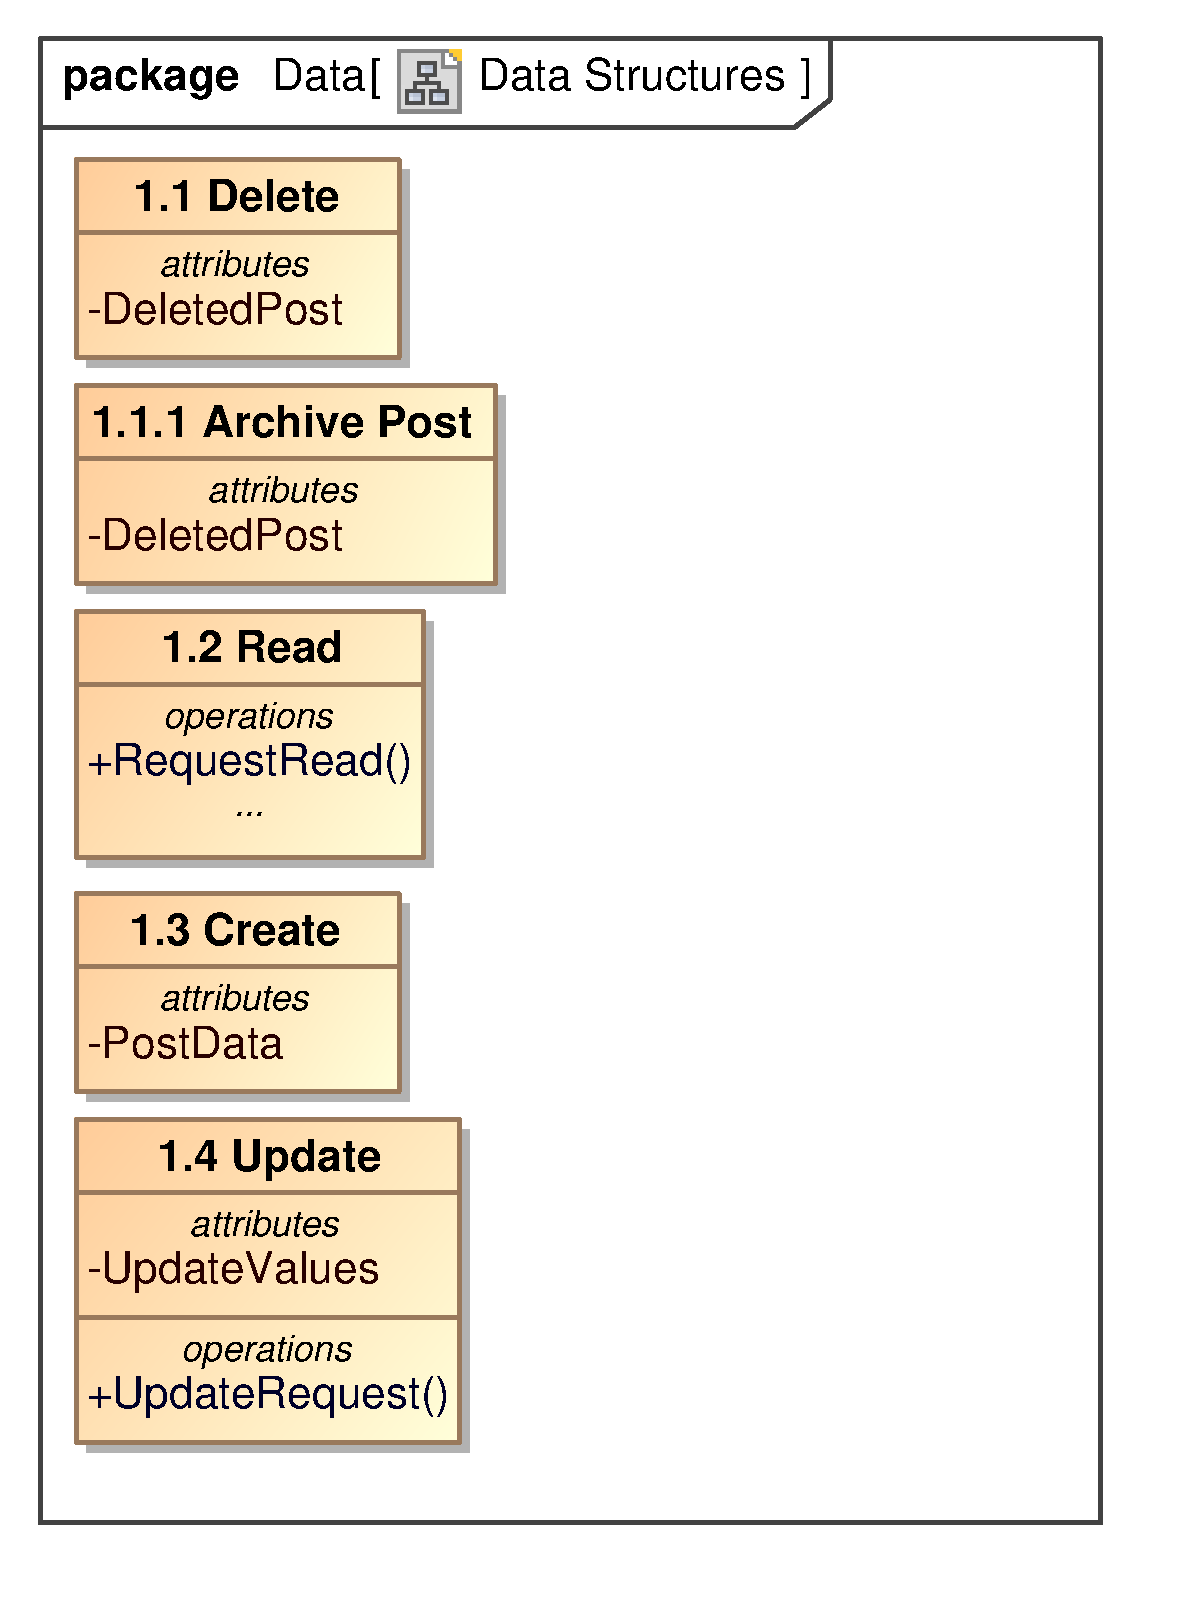
\includegraphics[scale=.4]{DataStructuresCRUD.eps}
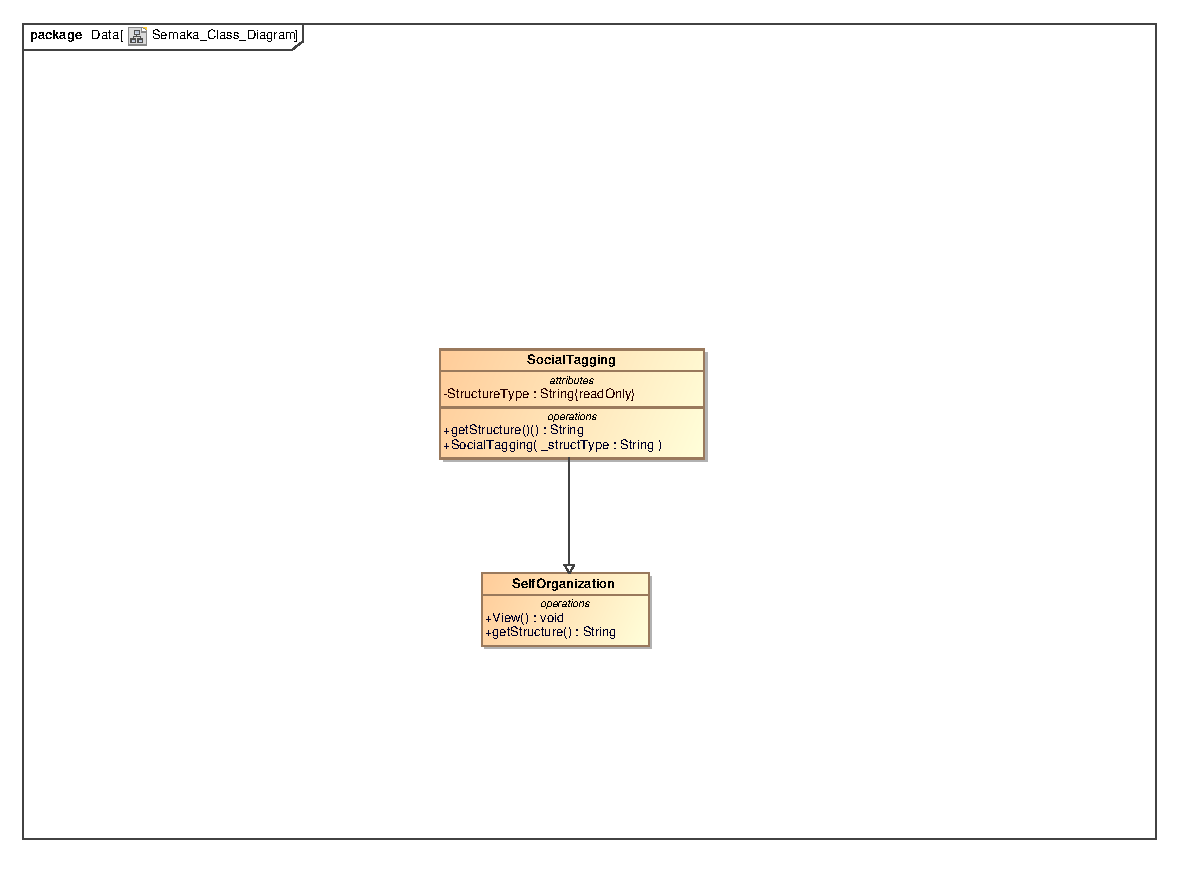
\includegraphics[scale=.4]{Semaka_Class_Diagram.eps}
\chapter{Required functionality} 							% Use Case Diagram
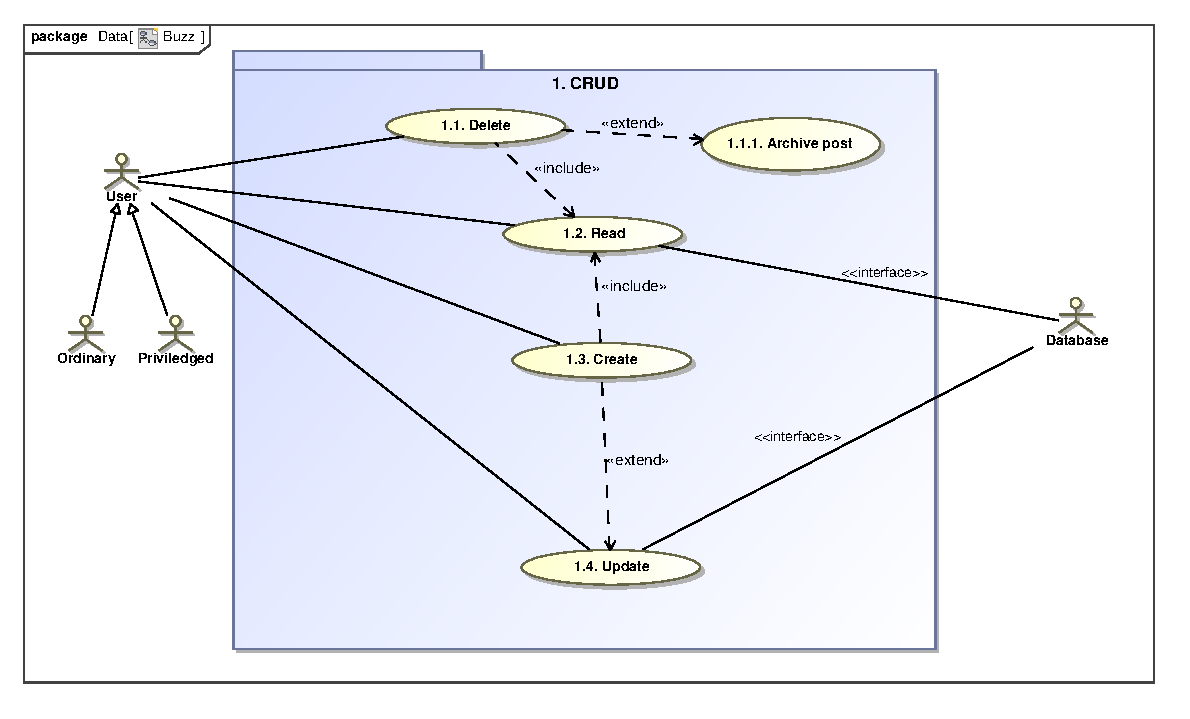
\includegraphics[scale=.9]{CRUDUSECASE.eps}\\
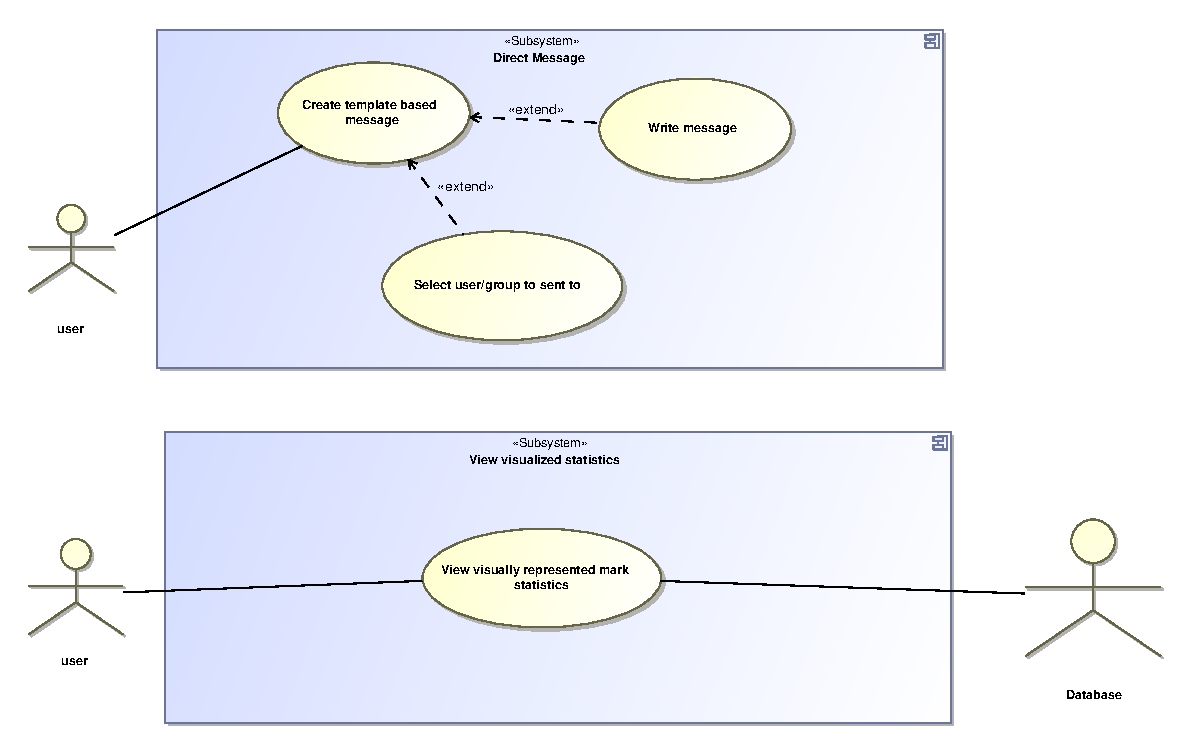
\includegraphics[scale=.9]{seanUC.eps}\\
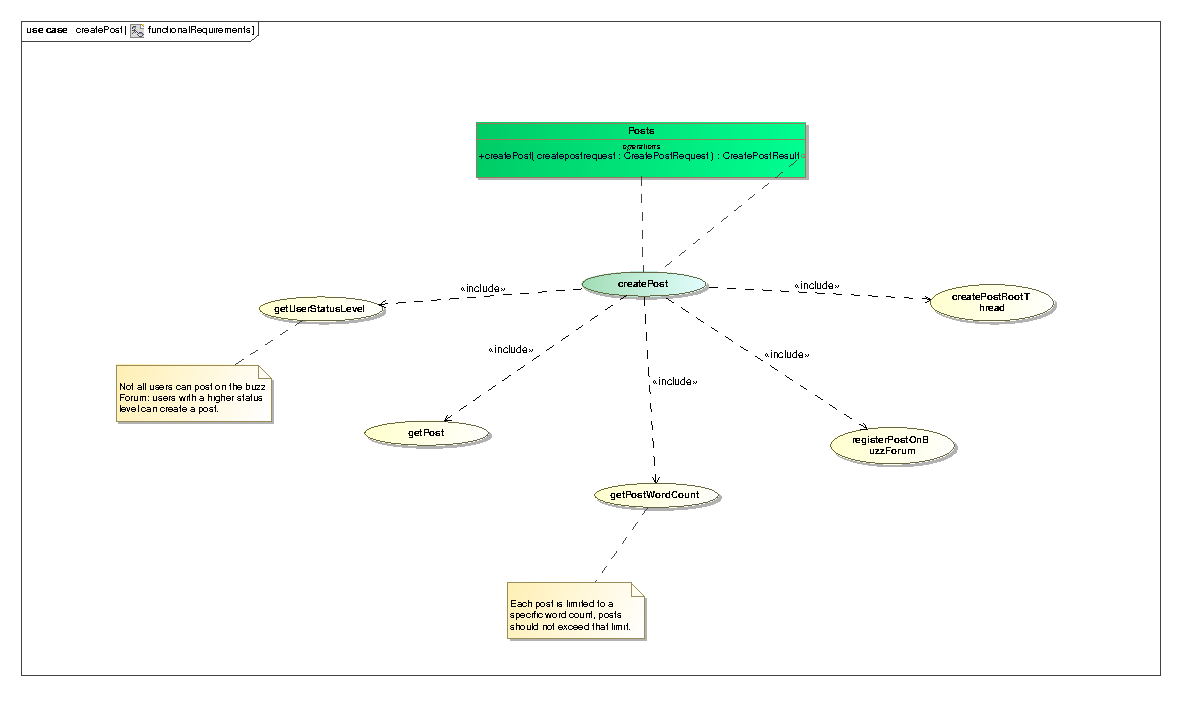
\includegraphics[scale=.9]{Shaun_functionalRequirements.eps}\\
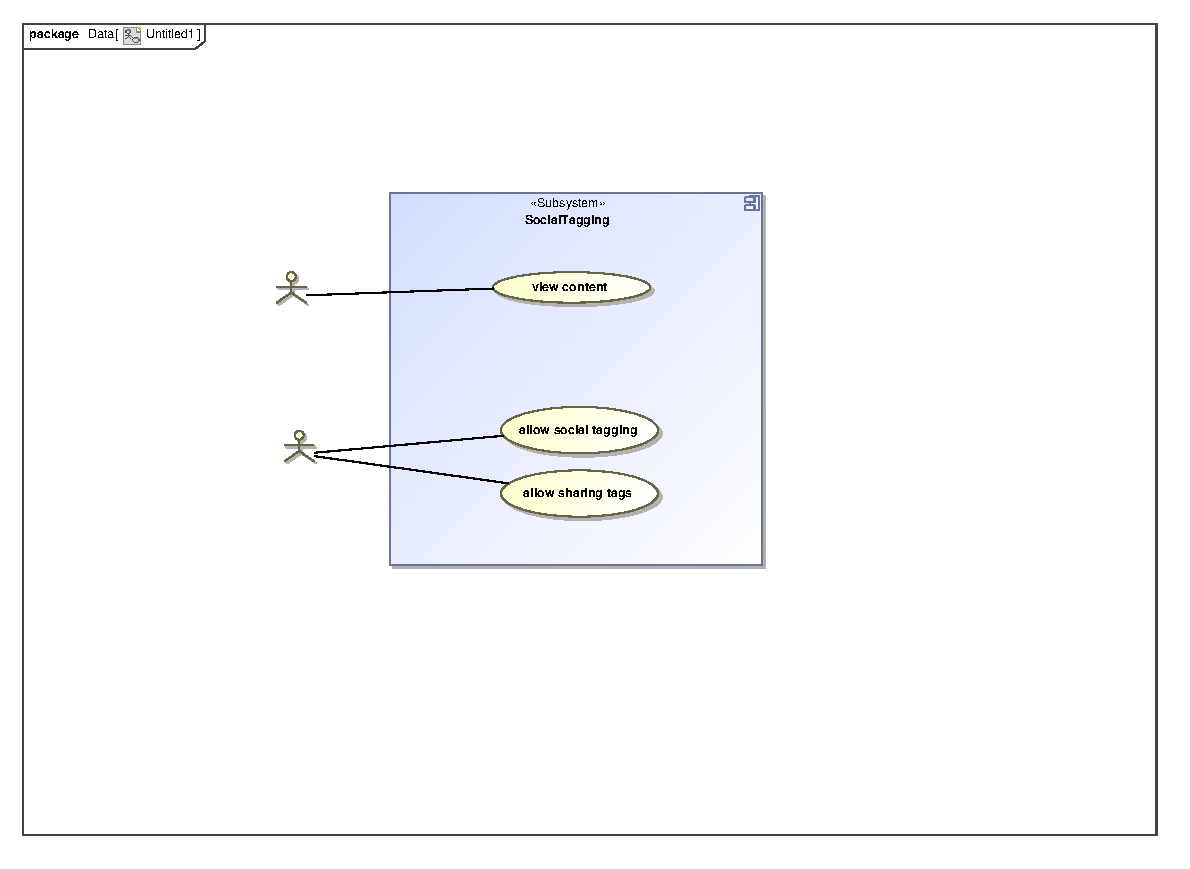
\includegraphics[scale=.9]{Semaka_Use_Case.eps}\\
\chapter{Process specifications}							% Activity Diagrams
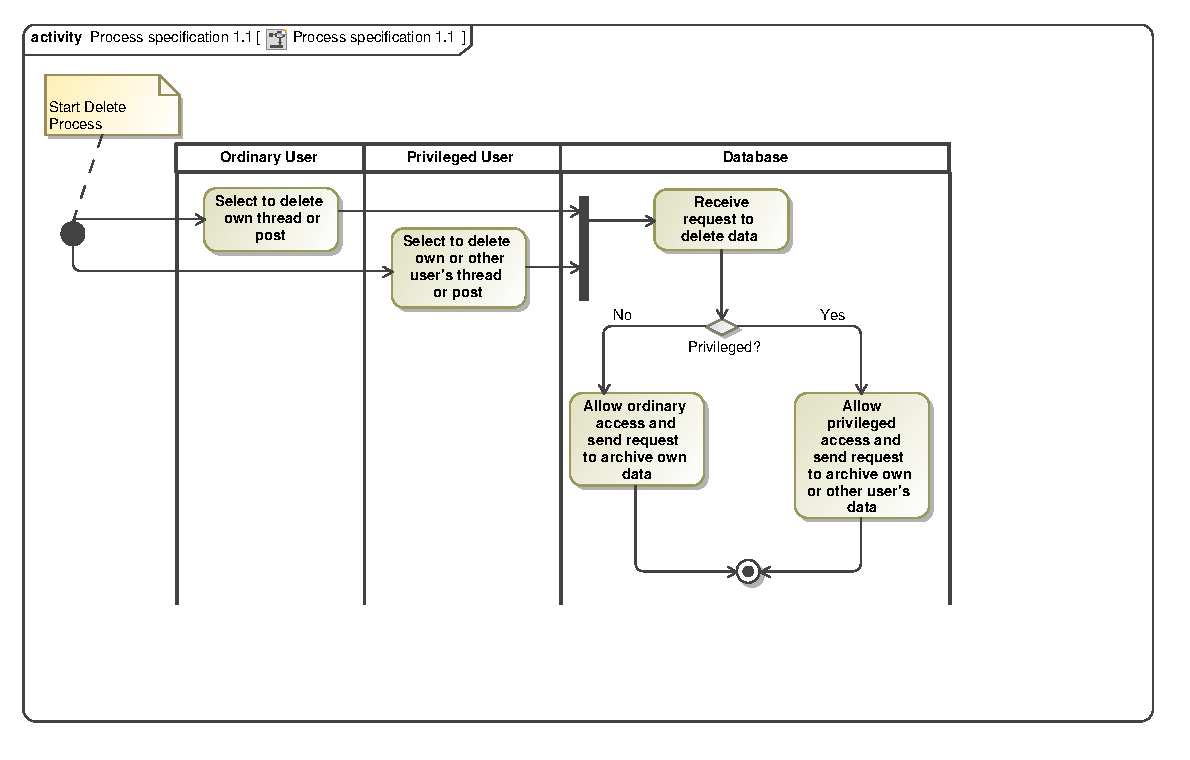
\includegraphics[scale=.9]{ProcessSpecificationCRUD1.eps}\\
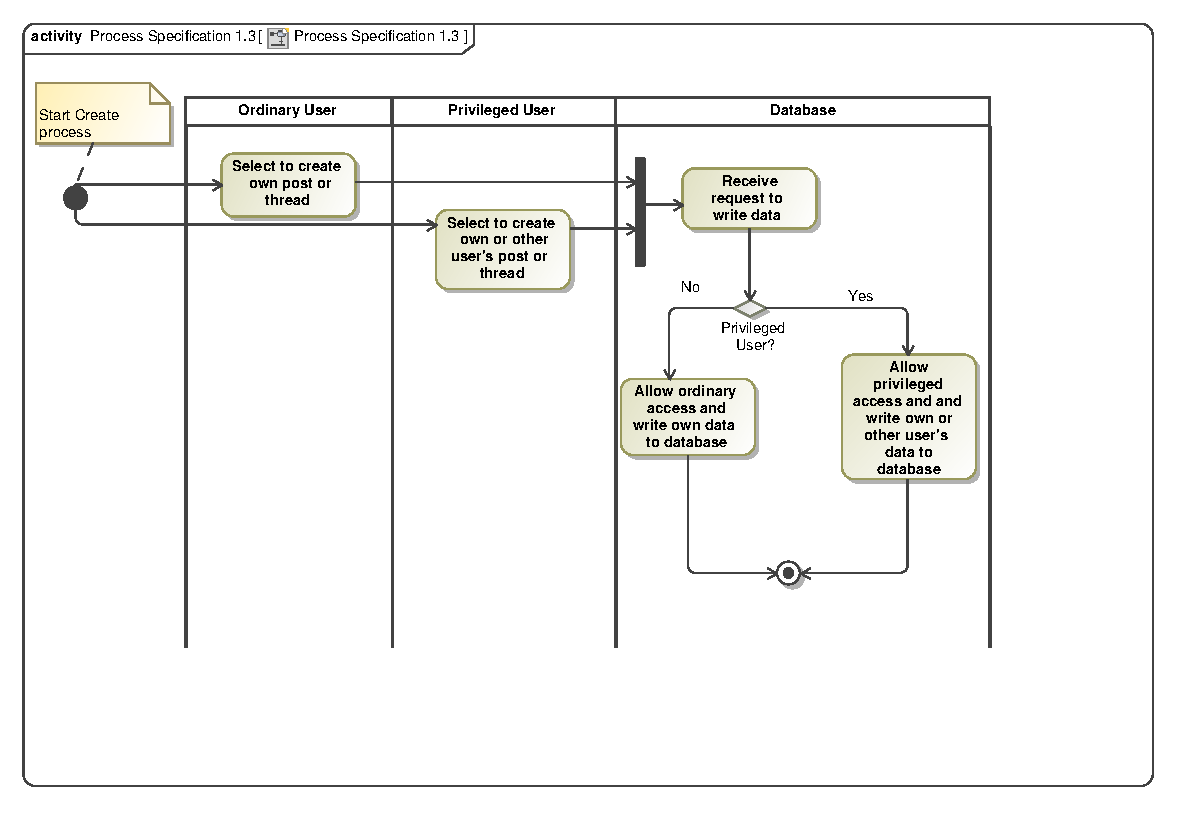
\includegraphics[scale=.9]{ProcessSpecificationCRUD3.eps}\\
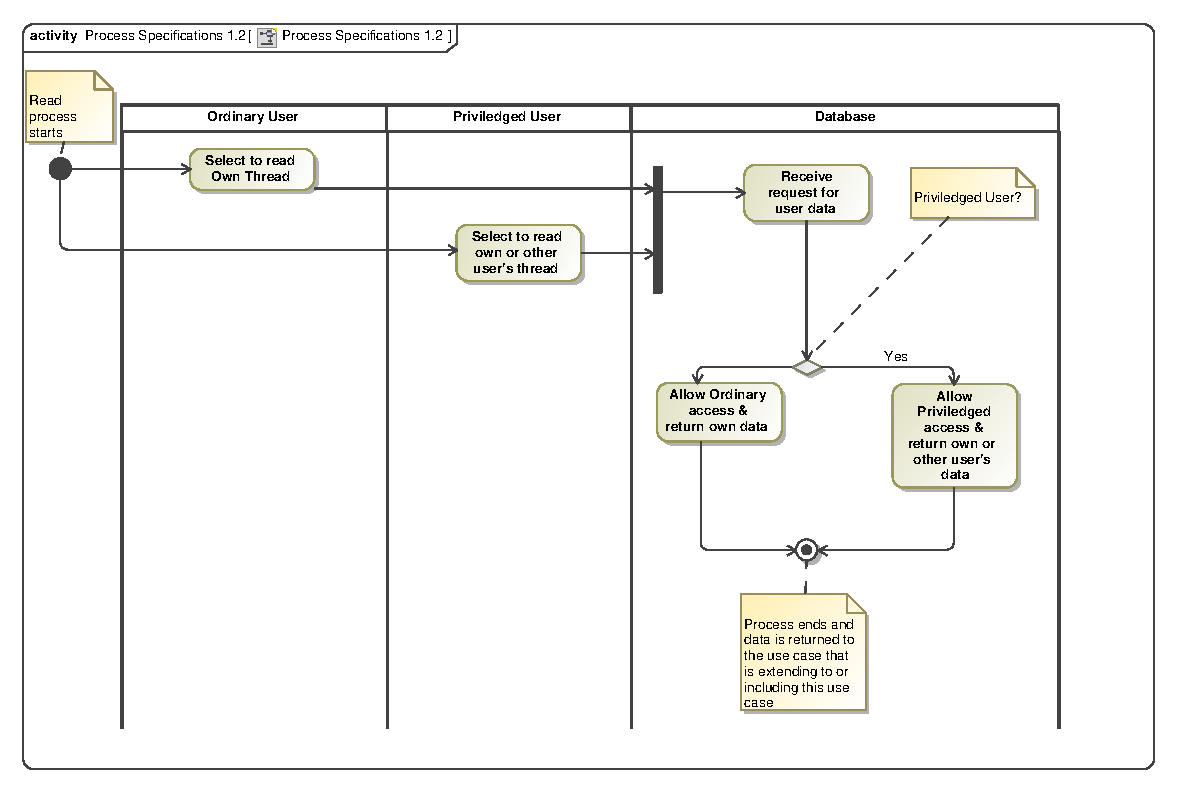
\includegraphics[scale=.9]{ProcessSpecificationsCRUD2.eps}\\
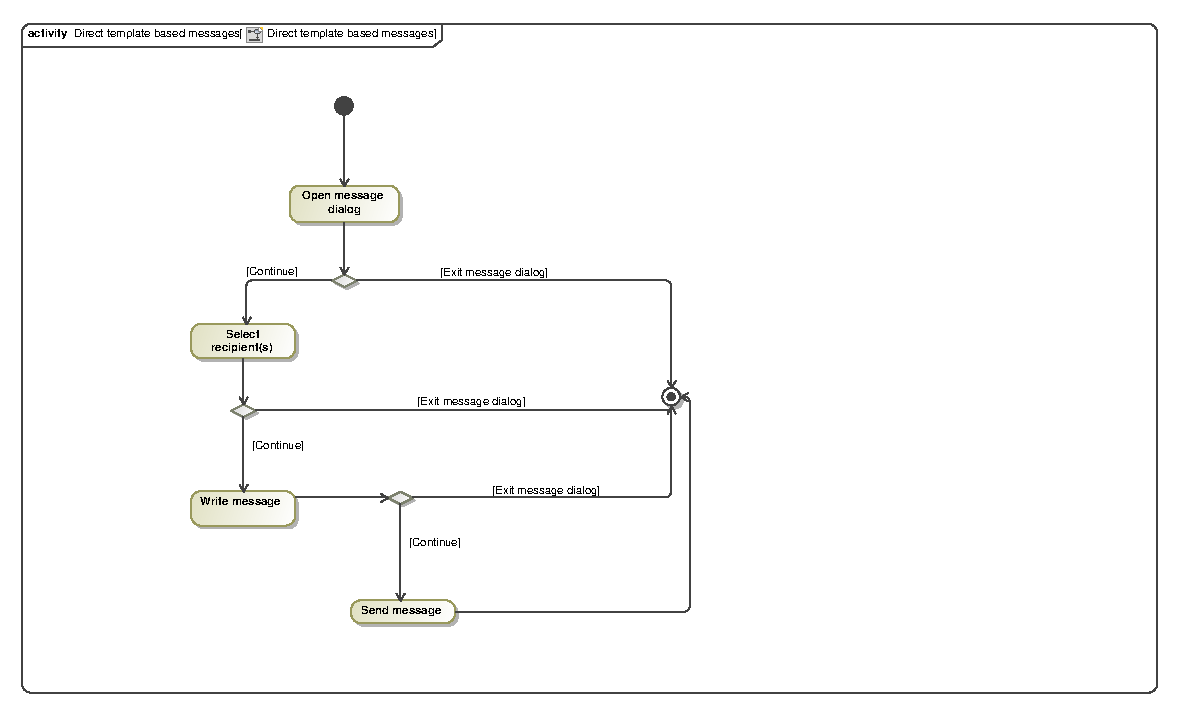
\includegraphics[scale=.9]{seanAC.eps}\\
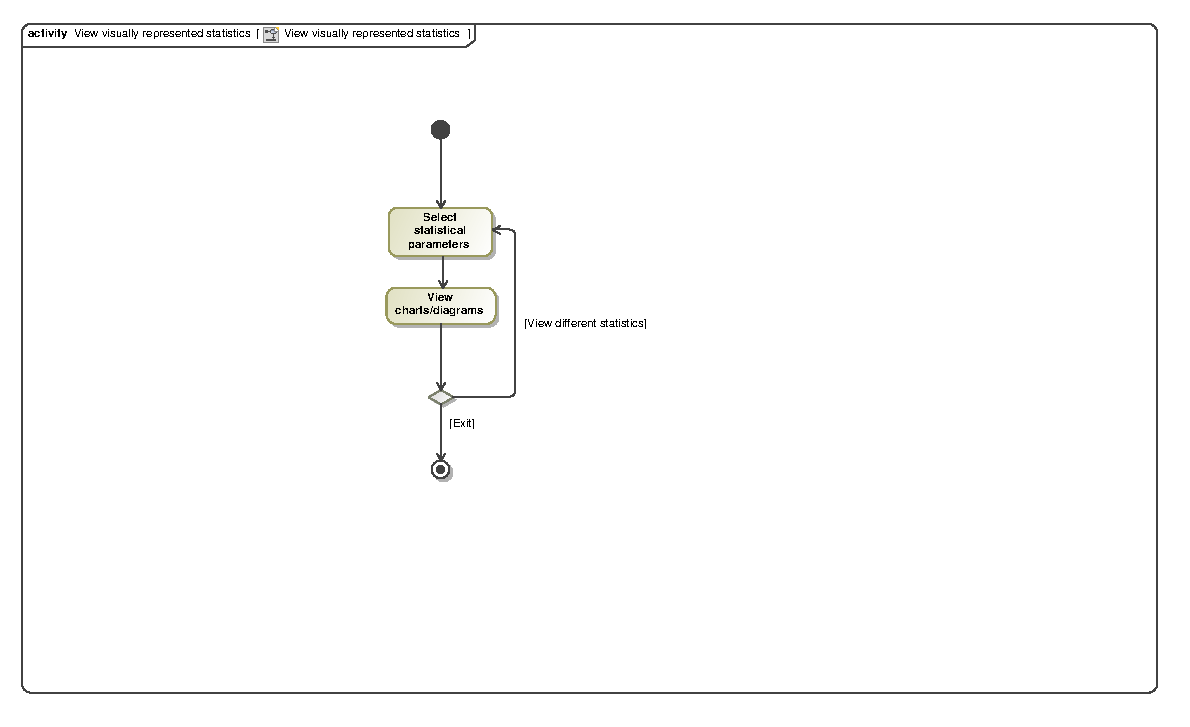
\includegraphics[scale=.9]{seanAC1.eps}\\
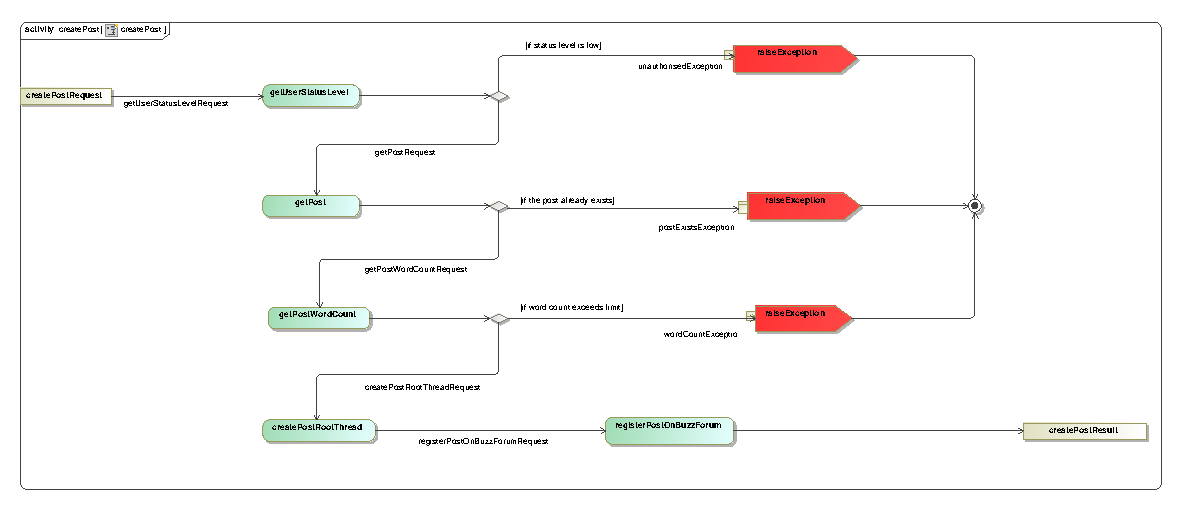
\includegraphics[scale=.9]{Shaun_activity.eps}\\
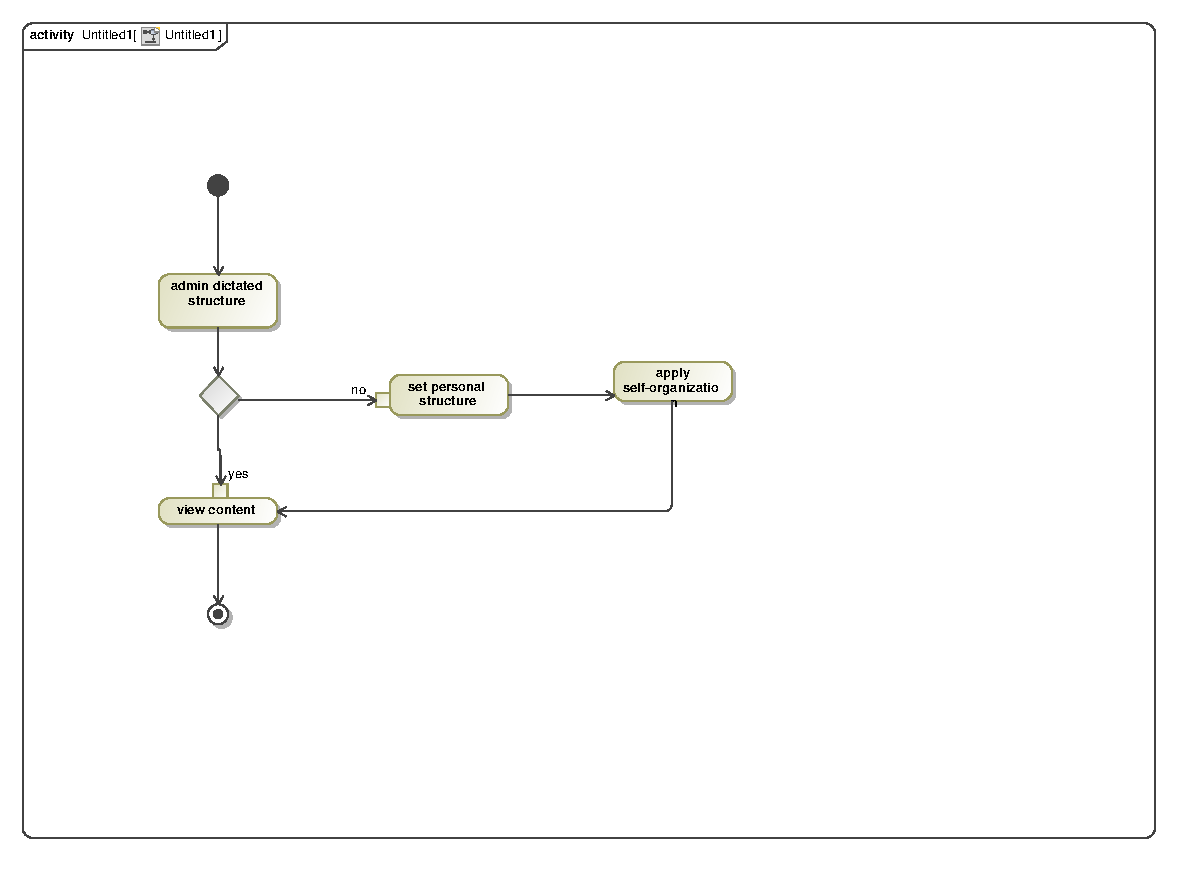
\includegraphics[scale=.9]{Semaka_Activity_Diagram.eps}\\
\chapter{Domain Model}   								% Class Diagras
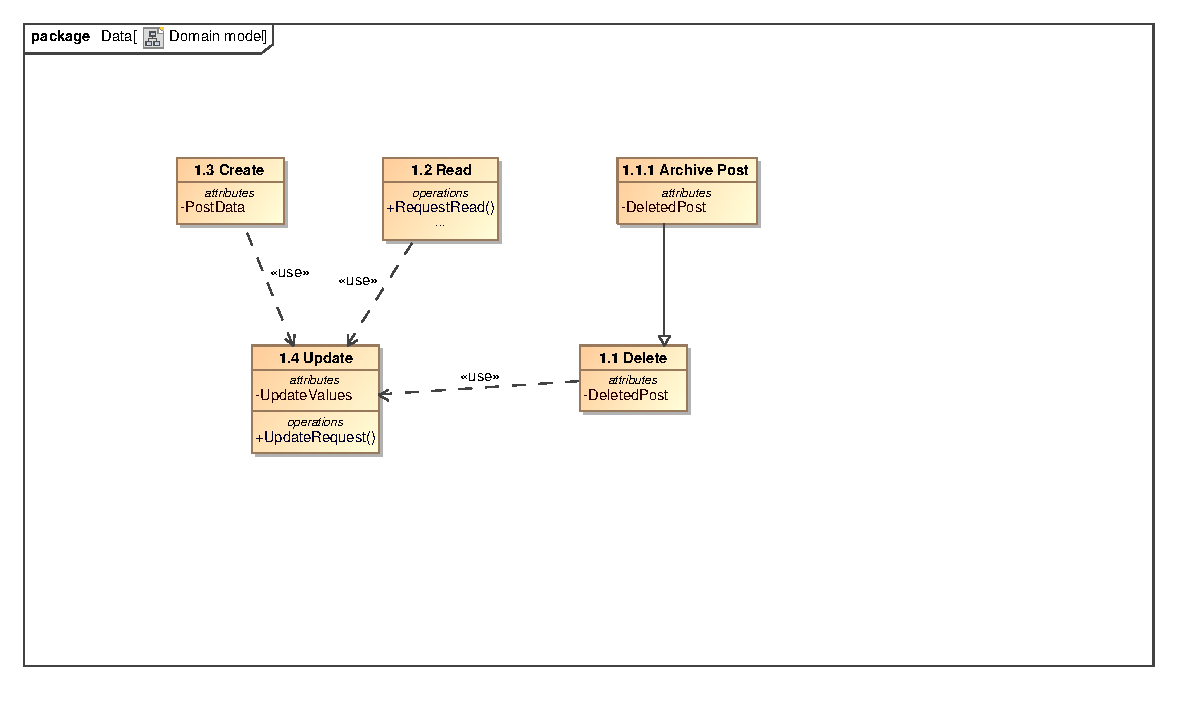
\includegraphics[scale=.9]{CRUDDomainModel.eps}\\
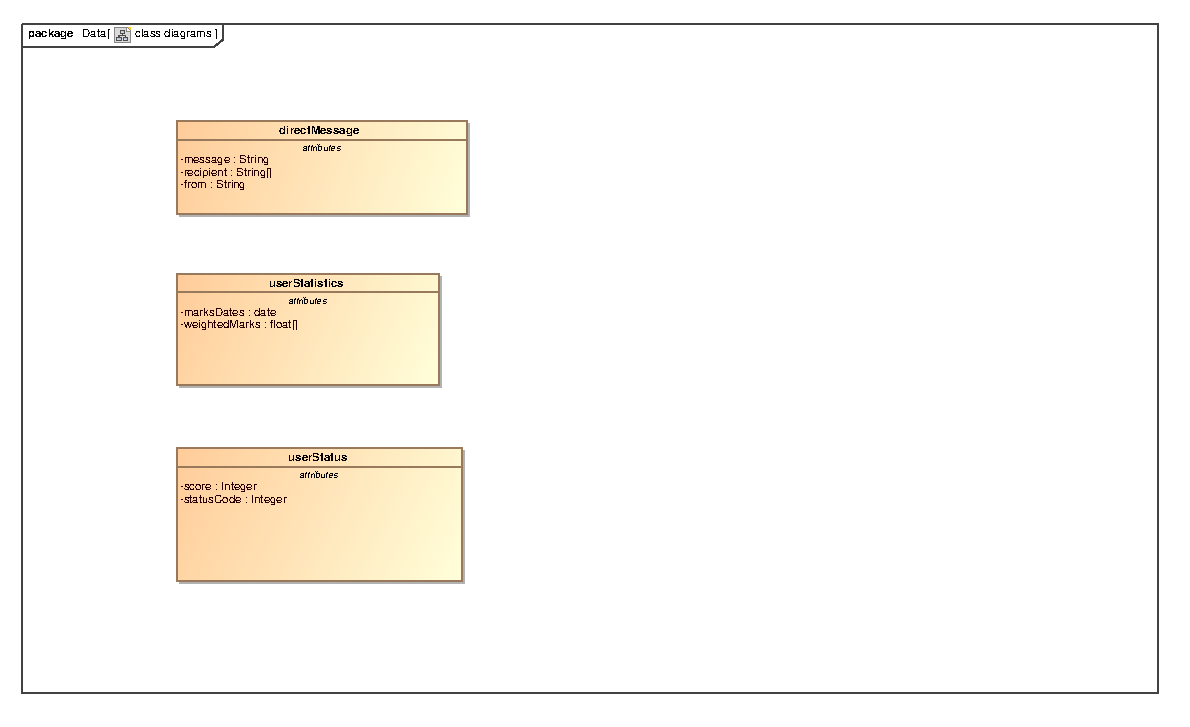
\includegraphics[scale=.9]{seanDM.eps}			
% add other chapters and sections to suit
\end{document}